



\begin{figure}[ht]
    \centering
    \caption{Uma frequência-resposta de um acelerômetro onde f\textsubscript{0} é a frequência natural e f\textsubscript{ref} é a frequência de referência.}
    \begin{center}
        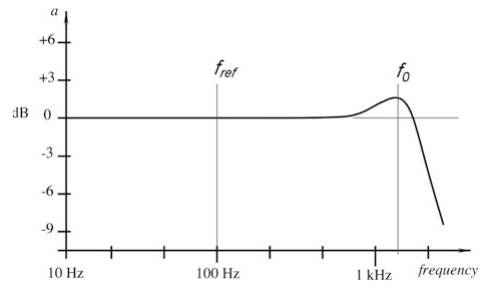
\includegraphics[width=0.7\textwidth]{img/print_grafico_resposta_do_acelerometro.png}
    \end{center}
    \vspace{-0.5cm}
    \legend{\ABNTEXfontereduzida \textbf{Fonte:} 
    \citeonline[p.~396]{ModernSensors}.}
    

    
    \label{fig:grafico_acelerometro}
\end{figure}